% \begin{figure}[ht!]
% 	\captionsetup[subfigure]{justification=justified}
% 	\centering
% 	\begin{subfigure}[t]{0.5\linewidth}
% 		\centering
% 		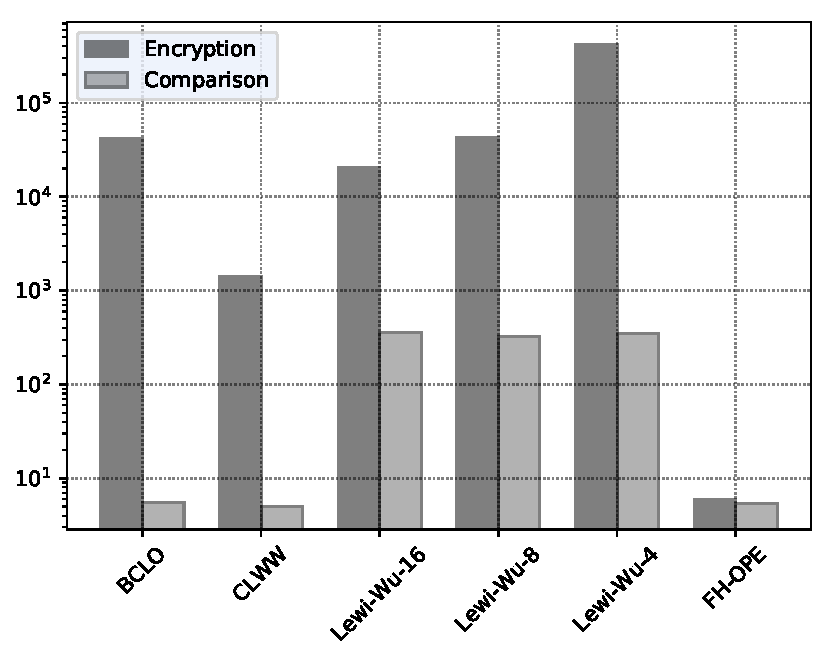
\includegraphics[width=\linewidth]{schemes-benchmark}
% 		\caption{Schemes benchmark (time in microseconds, log scale). Lewi-Wu parameter is the number of blocks.}
% 	\end{subfigure}%
% 	~ % chktex 39
% 	\begin{subfigure}[t]{0.5\linewidth}
% 		\centering
% 		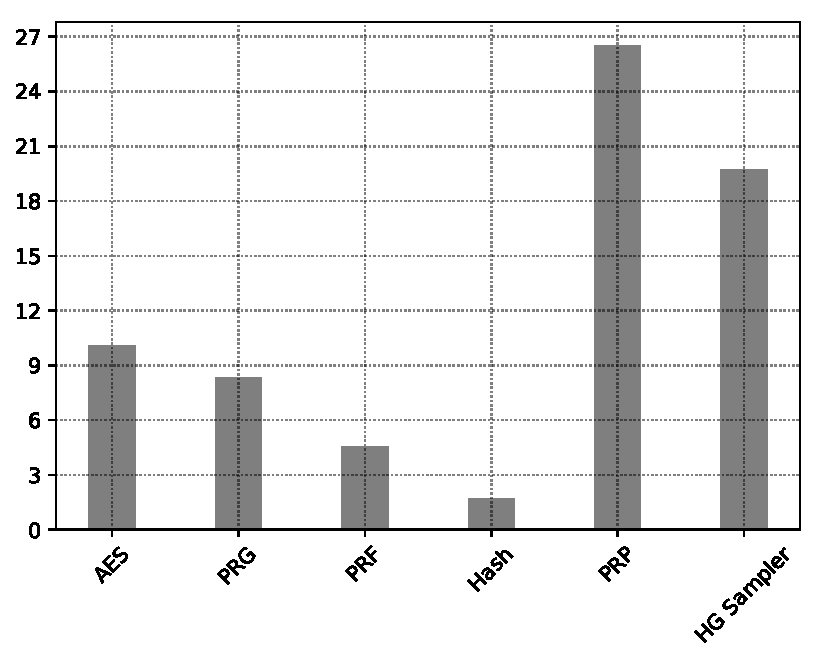
\includegraphics[width=\linewidth]{primitives-benchmark}
% 		\caption{Primitives benchmark (time in microseconds)}
% 	\end{subfigure}%
% 	\caption{Benchmarks of the schemes and primitives}\label{figure:benchmarks}
% \end{figure}

\begin{figure}[!ht]
	\centering
	\begin{minipage}[t]{0.48\columnwidth}
		\centering
		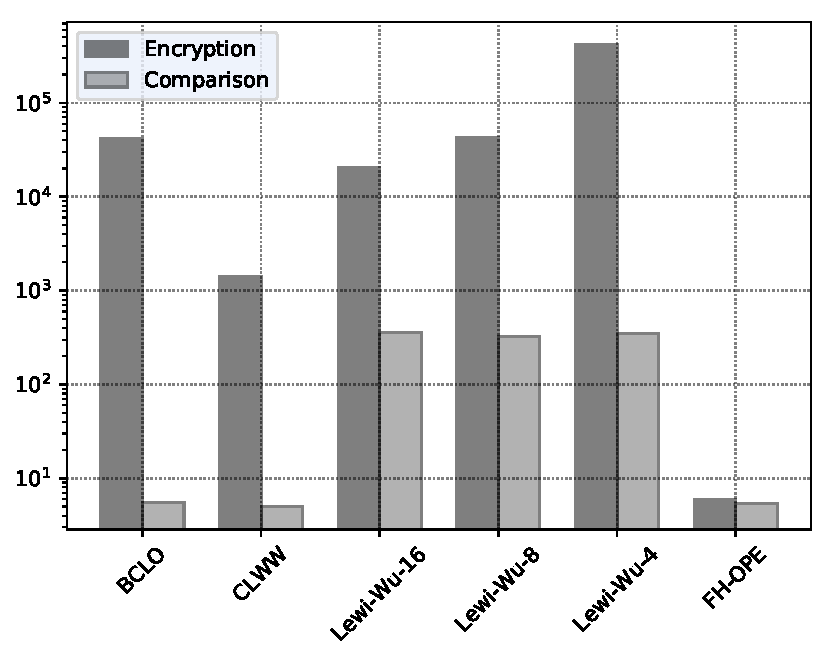
\includegraphics[width=\linewidth]{schemes-benchmark}
		\captionof{figure}{Schemes benchmark (time in microseconds, log scale). Lewi-Wu parameter is the number of blocks.}%
		\label{figure:benchmarks:schemes}
	\end{minipage}
	~ % chktex 39
	\begin{minipage}[t]{0.48\columnwidth}
		\centering
		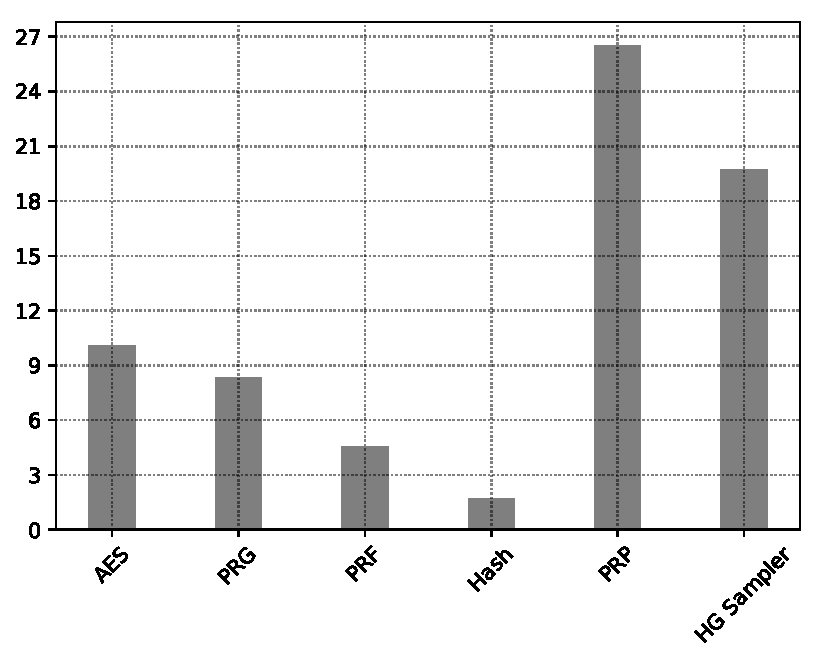
\includegraphics[width=\linewidth]{primitives-benchmark}
		\captionof{figure}{Primitives benchmark (time in microseconds)}%
		\label{figure:benchmarks:primitives}
	\end{minipage}
\end{figure}
